\documentclass{beamer}

\usetheme{CambridgeUS}
\beamertemplatenavigationsymbolsempty

\usepackage[utf8x]{inputenc}
\usepackage[T1]{fontenc}
\usepackage[francais]{babel}
\usepackage[autolanguage]{numprint}
\renewcommand*{\rmdefault}{fxb}
\usepackage{libertine}
\usepackage{lettrine}
\usepackage{hyperref}
\usepackage{wasysym}
\usepackage{listings}
\usepackage{xcolor}
\lstset{keywordstyle=\color{blue}, stringstyle=\color{green}}
\usepackage{amsmath}
\usepackage{wrapfig}
\usepackage{skak}
\usepackage{euler}
\usepackage{multicol}
\usepackage{graphicx}
\usepackage{tikz}
\usetikzlibrary{mindmap,trees}
\graphicspath{{./img/}}
\DeclareGraphicsExtensions{.png, .jpeg}


\renewcommand*\thesection{\arabic{section}}


\lstset{basicstyle=\footnotesize}

\title[Introduction à \LaTeX]{\LaTeX}
\subtitle{Pourquoi, comment.}
\institute{ASCII}
\date{7 novembre 2012}
\author[ASCII]{Rémi \textsc{Bois}
  \and Grégoire \textsc{Jadi}
  \and Hugo \textsc{Mougard}}


\begin{document}

\begin{frame}
  \maketitle  
\end{frame}

\begin{frame}
  \frametitle{Au menu ce soir}
  \tableofcontents
\end{frame}

\section{Pourquoi \LaTeX}

\begin{frame}
  \frametitle{What You See Is What You Get}
  \begin{figure}[H]
    \centering
    \includegraphics[width=9cm]{WYSIWYG}
    \caption{Libre Office}
    \label{fig:libre-office}
  \end{figure}
\end{frame}

\begin{frame}
  \frametitle{Avantages}
  \begin{itemize}
  \item prise en main facile
  \item adapté pour du \og pixel art \fg
  \item répandu chez les particuliers et les entreprises
  \end{itemize}
\end{frame}

\begin{frame}
  \frametitle{Inconvénients}
  \begin{itemize}
  \item devient vite dur à gérer (gros documents)
  \item utilisation correcte difficile
  \item des formats compliqués à utiliser (doc, docx, odt, \dots)
  \item souvent peu adapté pour les documents scientifiques
    (utilisation d'images, bibliographie \og à la main \fg)
  \end{itemize}
\end{frame}

\begin{frame}
  \frametitle{Principaux outils}
  \begin{itemize}
  \item Libre Office
  \item Word
  \item Pages
  \end{itemize}
\end{frame}

\begin{frame}
  \frametitle{What You See Is What You Mean}
  \begin{figure}[H]
    \centering
    \includegraphics[width=9cm]{WYSIWYM}
    \caption{Un document LaTeX}
    \label{fig:ex-LaTeX}
  \end{figure}
  \begin{figure}[H]
    \centering
    \includegraphics[width=6cm]{WYSIWYM-result}
    \caption{Le pdf qui lui correspond}
    \label{fig:ex-pdf}
  \end{figure}
\end{frame}

\begin{frame}
  \frametitle{Avantages}
  \begin{itemize}
  \item gestion des gros documents facile
  \item que du texte
  \item collaboration facile
  \item le résultat est créé automatiquement selon des règles de
    composition et typographie $\implies$ qualité du rendu
  \item bonne productivité une fois qu'on ma\^itrise l'outil
  \end{itemize}
\end{frame}

\begin{frame}
  \frametitle{Inconvénients}
  \begin{itemize}
  \item requiert un apprentissage
  \item le résultat est créé automatiquement selon des règles de
    composition et typographie $\implies$ pas de contr\^ole total
  \end{itemize}
\end{frame}

\begin{frame}
  \frametitle{Principal outil}
  \TeX{} et ses dérivés
\end{frame}

\begin{frame}
  \frametitle{Typographier des documents scientifiques}
  \begin{figure}[H]
    \centering
    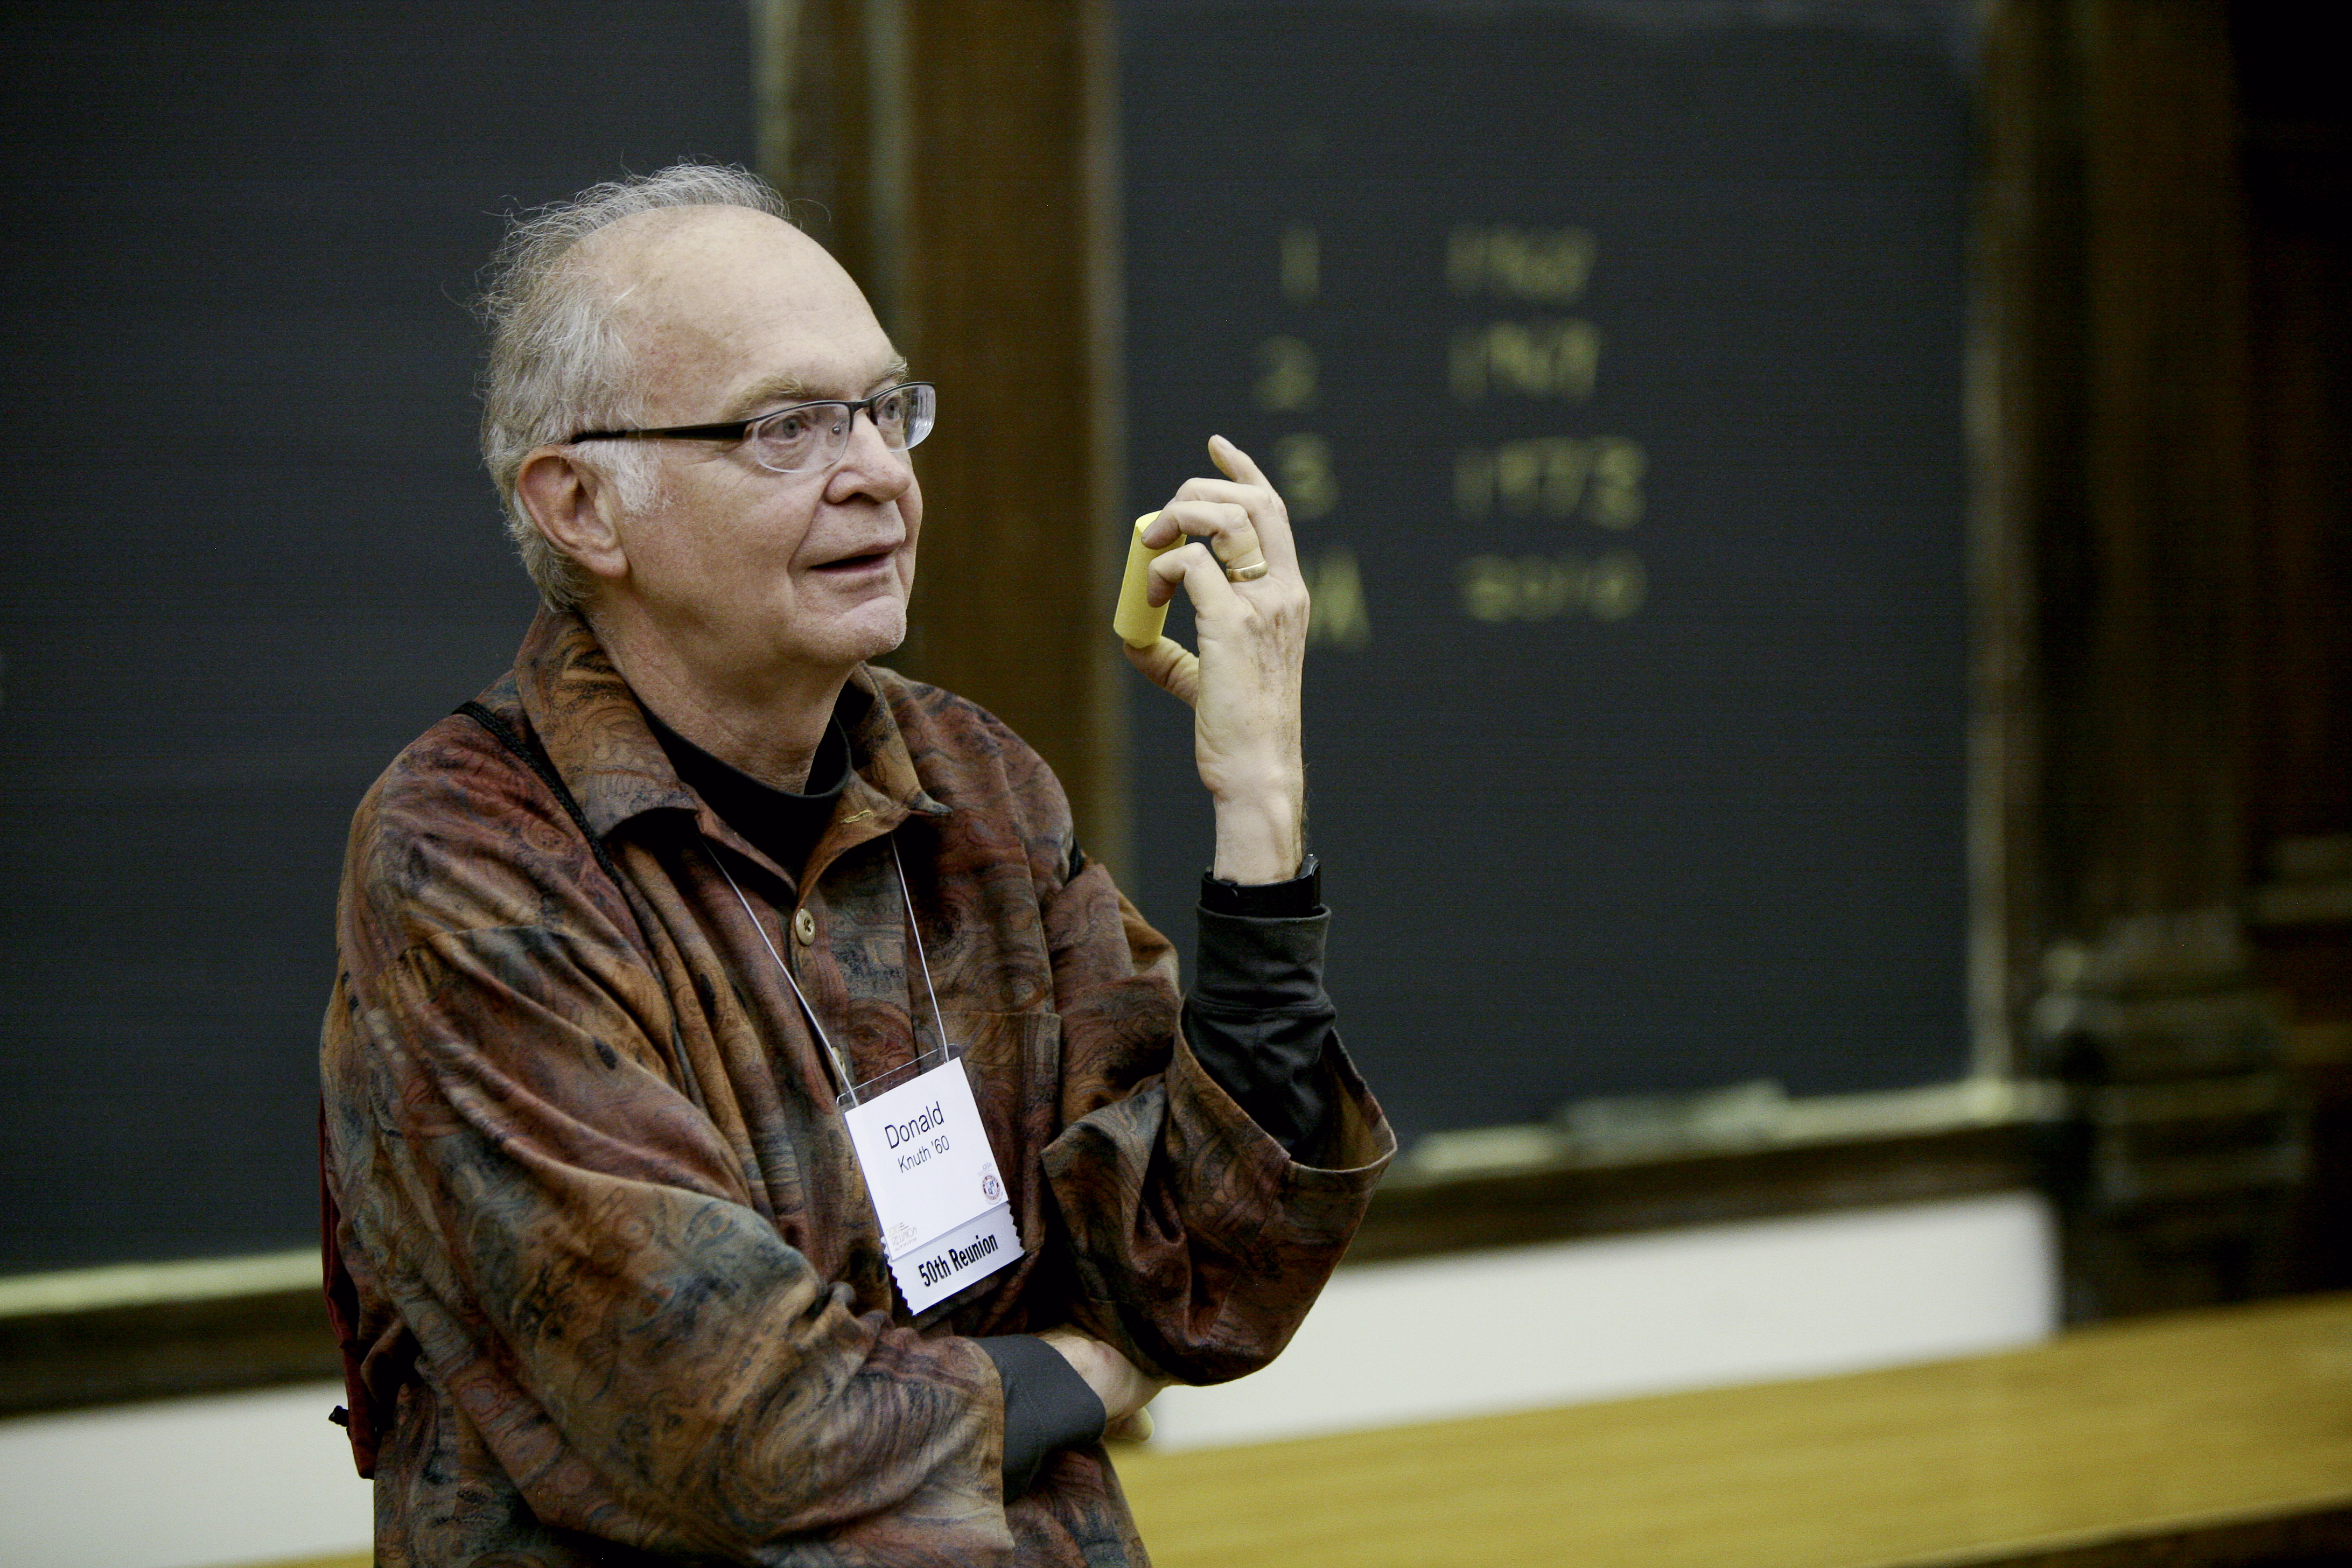
\includegraphics[width=7cm]{knuth}
    \caption{Donald Knuth}
    \label{fig:knuth}
  \end{figure}
\end{frame}

\begin{frame}
  \frametitle{Free comme dans \og free speech\fg}
  \begin{itemize}
  \item partage libre
  \item source disponible
  \item extensible
  \item gratuit
  \item ne dépend pas d'une entreprise (et de sa survie économique)
  \end{itemize}
\end{frame}

\begin{frame}
  \frametitle{Modulaire}
  \begin{itemize}
  \item système de paquets
  \item tout le monde peut contribuer
  \item dép\^ot commun (CTAN) où tout est centralisé
  \item quasi tout est paquets (le \og core\fg est minimal)
  \end{itemize}
\end{frame}

\begin{frame}
  \frametitle{La durabilité comme objectif majeur}
  \begin{itemize}
  \item features stables depuis la version 3 de \TeX.
  \item arithmétique à virgule fixe (portable sur tous les systèmes)
  \item format texte
  \item volonté politique de durabilité (compatibilité ascendante)
  \end{itemize}
\end{frame}

\begin{frame}
  \frametitle{Environnement de travail libre}
  Contrairement à Power Point ou Impress, on peut faire du \LaTeX{} de
  beaucoup de manières différentes.
\end{frame}
\section{Quelques exemples}
\begin{frame}[fragile]
  \frametitle{Programmes informatiques}
  
  Paquet \texttt{listings}
  
  \begin{block}{En Haskell}
\begin{lstlisting}[language=Haskell]
fibs :: [Integer]
fibs = 0 : 1 : zipWith (+) fibs (tail fibs)
\end{lstlisting}
  \end{block}
  \begin{block}{En C}
\begin{lstlisting}[language=C]
int
main(void)
{
    printf("%s", "Hello world!");
    return 0;
}
\end{lstlisting}
  \end{block}
\end{frame}

\begin{frame}
  \frametitle{Maths}
  Paquet \texttt{amsmath}, formules :

  \begin{equation*}
    f(x, µ, \sigma^2) = \frac{1}{\sigma\sqrt{2\pi}}e^{-\frac{1}{2}\left(\frac{x - µ}{\sigma}\right)^2}
  \end{equation*}

  Matrices :

  \[
  \begin{pmatrix}
    1 & 0 & 0 & 0 \\
    0 & 1 & 0 & 0 \\
    0 & 0 & 1 & 0 \\
    0 & 0 & 0 & 1 \\
  \end{pmatrix}
  \]

  Et \textbf{beaucoup} d'autres choses\dots
\end{frame}

\begin{frame}
  \frametitle{Figures}
  Paquet \texttt{Tikz}
  
  \scalebox{0.5}{
    \begin{tikzpicture}
      \path[mindmap,concept color=black,text=white]
        node[concept] {Computer Science}
        [clockwise from=0]
        child[concept color=green!50!black] {
          node[concept] {practical}
          [clockwise from=90]
          child { node[concept] {algorithms} }
          child { node[concept] {data structures} }
          child { node[concept] {pro\-gramming languages} }
          child { node[concept] {software engineer\-ing} }
        }  
        child[concept color=blue] {
          node[concept] {applied}
          [clockwise from=-30]
          child { node[concept] {databases} }
          child { node[concept] {WWW} }
        }
        child[concept color=red] { node[concept] {technical} }
        child[concept color=orange] { node[concept] {theoretical}
      };
    \end{tikzpicture}
  }
\end{frame}

\begin{frame}
  \frametitle{Partitions de musique}
  \begin{figure}[H]
    \centering
    \includegraphics[width=10cm]{lilypond}
    \caption{Partition avec Lilypond}
    \label{fig:lilypond}
  \end{figure}
\end{frame}

\begin{frame}[fragile]
  \frametitle{Jeux}
  \newgame
  \notationoff
  \begin{multicols}{2}
    Coup du berger :
    
    \mainline{1. e4 e5}   \\
    \mainline{2. Bc4 Bc5} \\
    \mainline{3. Qf3 Nc6} \\
    \mainline{4. Qf7#}
    \columnbreak
    \showboard
  \end{multicols}
\end{frame}

\section{Comment ça marche}

\begin{frame}
  \frametitle{On bosse un peu}
  Une vraie démo maintenant\dots (sans l'effet démo hopefully)
\end{frame}

\begin{frame}[allowframebreaks]
  \frametitle{Bibliographie}
  \nocite{texse}
  \nocite{latex}
  \nocite{lshort}
  \nocite{comprehensive}
  \nocite{newsgroup}
  \nocite{mathguide}
  \nocite{ctan}
  \bibliographystyle{plain}
  \bibliography{biblio}
\end{frame}
\end{document}
